% Options for packages loaded elsewhere
\PassOptionsToPackage{unicode}{hyperref}
\PassOptionsToPackage{hyphens}{url}
\PassOptionsToPackage{dvipsnames,svgnames,x11names}{xcolor}
%
\documentclass[
  letterpaper,
  DIV=11,
  numbers=noendperiod]{scrreprt}

\usepackage{amsmath,amssymb}
\usepackage{iftex}
\ifPDFTeX
  \usepackage[T1]{fontenc}
  \usepackage[utf8]{inputenc}
  \usepackage{textcomp} % provide euro and other symbols
\else % if luatex or xetex
  \usepackage{unicode-math}
  \defaultfontfeatures{Scale=MatchLowercase}
  \defaultfontfeatures[\rmfamily]{Ligatures=TeX,Scale=1}
\fi
\usepackage{lmodern}
\ifPDFTeX\else  
    % xetex/luatex font selection
\fi
% Use upquote if available, for straight quotes in verbatim environments
\IfFileExists{upquote.sty}{\usepackage{upquote}}{}
\IfFileExists{microtype.sty}{% use microtype if available
  \usepackage[]{microtype}
  \UseMicrotypeSet[protrusion]{basicmath} % disable protrusion for tt fonts
}{}
\makeatletter
\@ifundefined{KOMAClassName}{% if non-KOMA class
  \IfFileExists{parskip.sty}{%
    \usepackage{parskip}
  }{% else
    \setlength{\parindent}{0pt}
    \setlength{\parskip}{6pt plus 2pt minus 1pt}}
}{% if KOMA class
  \KOMAoptions{parskip=half}}
\makeatother
\usepackage{xcolor}
\setlength{\emergencystretch}{3em} % prevent overfull lines
\setcounter{secnumdepth}{5}
% Make \paragraph and \subparagraph free-standing
\makeatletter
\ifx\paragraph\undefined\else
  \let\oldparagraph\paragraph
  \renewcommand{\paragraph}{
    \@ifstar
      \xxxParagraphStar
      \xxxParagraphNoStar
  }
  \newcommand{\xxxParagraphStar}[1]{\oldparagraph*{#1}\mbox{}}
  \newcommand{\xxxParagraphNoStar}[1]{\oldparagraph{#1}\mbox{}}
\fi
\ifx\subparagraph\undefined\else
  \let\oldsubparagraph\subparagraph
  \renewcommand{\subparagraph}{
    \@ifstar
      \xxxSubParagraphStar
      \xxxSubParagraphNoStar
  }
  \newcommand{\xxxSubParagraphStar}[1]{\oldsubparagraph*{#1}\mbox{}}
  \newcommand{\xxxSubParagraphNoStar}[1]{\oldsubparagraph{#1}\mbox{}}
\fi
\makeatother


\providecommand{\tightlist}{%
  \setlength{\itemsep}{0pt}\setlength{\parskip}{0pt}}\usepackage{longtable,booktabs,array}
\usepackage{calc} % for calculating minipage widths
% Correct order of tables after \paragraph or \subparagraph
\usepackage{etoolbox}
\makeatletter
\patchcmd\longtable{\par}{\if@noskipsec\mbox{}\fi\par}{}{}
\makeatother
% Allow footnotes in longtable head/foot
\IfFileExists{footnotehyper.sty}{\usepackage{footnotehyper}}{\usepackage{footnote}}
\makesavenoteenv{longtable}
\usepackage{graphicx}
\makeatletter
\def\maxwidth{\ifdim\Gin@nat@width>\linewidth\linewidth\else\Gin@nat@width\fi}
\def\maxheight{\ifdim\Gin@nat@height>\textheight\textheight\else\Gin@nat@height\fi}
\makeatother
% Scale images if necessary, so that they will not overflow the page
% margins by default, and it is still possible to overwrite the defaults
% using explicit options in \includegraphics[width, height, ...]{}
\setkeys{Gin}{width=\maxwidth,height=\maxheight,keepaspectratio}
% Set default figure placement to htbp
\makeatletter
\def\fps@figure{htbp}
\makeatother
% definitions for citeproc citations
\NewDocumentCommand\citeproctext{}{}
\NewDocumentCommand\citeproc{mm}{%
  \begingroup\def\citeproctext{#2}\cite{#1}\endgroup}
\makeatletter
 % allow citations to break across lines
 \let\@cite@ofmt\@firstofone
 % avoid brackets around text for \cite:
 \def\@biblabel#1{}
 \def\@cite#1#2{{#1\if@tempswa , #2\fi}}
\makeatother
\newlength{\cslhangindent}
\setlength{\cslhangindent}{1.5em}
\newlength{\csllabelwidth}
\setlength{\csllabelwidth}{3em}
\newenvironment{CSLReferences}[2] % #1 hanging-indent, #2 entry-spacing
 {\begin{list}{}{%
  \setlength{\itemindent}{0pt}
  \setlength{\leftmargin}{0pt}
  \setlength{\parsep}{0pt}
  % turn on hanging indent if param 1 is 1
  \ifodd #1
   \setlength{\leftmargin}{\cslhangindent}
   \setlength{\itemindent}{-1\cslhangindent}
  \fi
  % set entry spacing
  \setlength{\itemsep}{#2\baselineskip}}}
 {\end{list}}
\usepackage{calc}
\newcommand{\CSLBlock}[1]{\hfill\break\parbox[t]{\linewidth}{\strut\ignorespaces#1\strut}}
\newcommand{\CSLLeftMargin}[1]{\parbox[t]{\csllabelwidth}{\strut#1\strut}}
\newcommand{\CSLRightInline}[1]{\parbox[t]{\linewidth - \csllabelwidth}{\strut#1\strut}}
\newcommand{\CSLIndent}[1]{\hspace{\cslhangindent}#1}

\KOMAoption{captions}{tableheading}
\makeatletter
\@ifpackageloaded{bookmark}{}{\usepackage{bookmark}}
\makeatother
\makeatletter
\@ifpackageloaded{caption}{}{\usepackage{caption}}
\AtBeginDocument{%
\ifdefined\contentsname
  \renewcommand*\contentsname{Table of contents}
\else
  \newcommand\contentsname{Table of contents}
\fi
\ifdefined\listfigurename
  \renewcommand*\listfigurename{List of Figures}
\else
  \newcommand\listfigurename{List of Figures}
\fi
\ifdefined\listtablename
  \renewcommand*\listtablename{List of Tables}
\else
  \newcommand\listtablename{List of Tables}
\fi
\ifdefined\figurename
  \renewcommand*\figurename{Fig.}
\else
  \newcommand\figurename{Fig.}
\fi
\ifdefined\tablename
  \renewcommand*\tablename{Tabela}
\else
  \newcommand\tablename{Tabela}
\fi
}
\@ifpackageloaded{float}{}{\usepackage{float}}
\floatstyle{ruled}
\@ifundefined{c@chapter}{\newfloat{codelisting}{h}{lop}}{\newfloat{codelisting}{h}{lop}[chapter]}
\floatname{codelisting}{Listing}
\newcommand*\listoflistings{\listof{codelisting}{List of Listings}}
\makeatother
\makeatletter
\makeatother
\makeatletter
\@ifpackageloaded{caption}{}{\usepackage{caption}}
\@ifpackageloaded{subcaption}{}{\usepackage{subcaption}}
\makeatother

\ifLuaTeX
  \usepackage{selnolig}  % disable illegal ligatures
\fi
\usepackage{bookmark}

\IfFileExists{xurl.sty}{\usepackage{xurl}}{} % add URL line breaks if available
\urlstyle{same} % disable monospaced font for URLs
\hypersetup{
  pdftitle={Introdução à Análise de Dados em Arqueologia},
  colorlinks=true,
  linkcolor={blue},
  filecolor={Maroon},
  citecolor={Blue},
  urlcolor={Blue},
  pdfcreator={LaTeX via pandoc}}


\title{Introdução à Análise de Dados em Arqueologia}
\author{}
\date{}

\begin{document}
\maketitle

\renewcommand*\contentsname{Table of contents}
{
\hypersetup{linkcolor=}
\setcounter{tocdepth}{2}
\tableofcontents
}

\bookmarksetup{startatroot}

\chapter*{Sobre este livro}\label{sobre-este-livro}
\addcontentsline{toc}{chapter}{Sobre este livro}

\markboth{Sobre este livro}{Sobre este livro}

Lorem ipsum dolor sit amet, consectetur adipiscing elit. Nam venenatis
mauris quis turpis aliquet varius vel vel elit. Sed euismod ullamcorper
dictum. Ut velit nisl, ultrices mattis condimentum vel, sollicitudin nec
neque. Maecenas blandit molestie fringilla. Nullam enim nisl, rhoncus eu
ex vel, euismod hendrerit libero. Aliquam tempor, augue ac lacinia
blandit, eros magna pellentesque tellus, et blandit lacus leo in eros.
Nunc mattis libero nec gravida vehicula.

Vestibulum congue condimentum magna posuere mattis. Morbi non eleifend
sapien, ac auctor ipsum. Proin eu tortor odio. Sed a facilisis nisl.
Curabitur sed mauris ultrices, lobortis est et, placerat sem.
Pellentesque dapibus mollis nisi vel pulvinar. In hac habitasse platea
dictumst. Phasellus laoreet elit at dictum rutrum. Suspendisse porttitor
efficitur lobortis.

Maecenas ornare tristique quam, viverra sagittis libero tincidunt vel.
Etiam arcu mi, gravida eu efficitur semper, malesuada et mi. Duis
vestibulum mollis felis non lacinia. Duis sodales lacus sed placerat
mollis. Mauris diam lacus, euismod at eros eu, tempus viverra magna.
Vestibulum et dictum sapien, ut fringilla augue. In ac magna augue.
Phasellus venenatis eleifend nulla. Ut vitae justo nisi. Morbi pharetra
turpis quis massa ullamcorper, at placerat odio pharetra. Proin mi erat,
vulputate eu augue ut, commodo condimentum ante.

Nullam lobortis ultricies commodo. Mauris posuere pretium ultrices. Duis
nunc massa, semper ut odio porta, porta ornare eros. In hac habitasse
platea dictumst. Interdum et malesuada fames ac ante ipsum primis in
faucibus. Etiam ultrices nibh tellus, sit amet viverra ante placerat in.
Vestibulum a enim efficitur, commodo ipsum eu, ullamcorper purus.
Vivamus vitae placerat purus, vitae scelerisque dui.

Aenean eleifend, ex et egestas maximus, neque ipsum facilisis magna, at
sodales risus velit congue ante. Duis ultrices libero in velit euismod,
vitae ultricies ipsum varius. Etiam mattis in lacus eget semper. Donec
nec tellus velit. Nam cursus eros id condimentum iaculis. Phasellus quis
odio ac diam aliquam facilisis. Maecenas luctus laoreet eleifend.

\section*{Agradecimentos}\label{agradecimentos}
\addcontentsline{toc}{section}{Agradecimentos}

\markright{Agradecimentos}

\bookmarksetup{startatroot}

\chapter*{Preâmbulo}\label{preuxe2mbulo}
\addcontentsline{toc}{chapter}{Preâmbulo}

\markboth{Preâmbulo}{Preâmbulo}

Em termos gerais, a Arqueologia pré-década de 1960 estava
maioritariamente baseada numa descrição empírica da cultura material, o
que incluía acreditar que uma grande quantidade de dados ``falariam''
sempre por si próprios. Os padrões emergiriam do estudo descritivo de
coleções de dados, permitindo que cerâmicas, ferramentas em pedra ou
estruturas arqueológicas fizessem sentido quando agrupadas segundo
determinadas características, às quais depois eram atribuídos limites
espaciais e temporais por meio do conceito normativo Childeano de
``Cultura Arqueológica''
\href{https://www.zotero.org/google-docs/?gebJdf}{(Johnson, 2019)}.
Devido a este contexto teórico, os dados eram tidos como adquiridos pela
maior parte dos arqueólogos e o processo de observação, registo e
interpretação necessitava de pouca, se não mesmo nenhuma, justificação
\href{https://www.zotero.org/google-docs/?eiFPcA}{(Lock, 2003)}.

As mudanças com a Nova Arqueologia, iniciadas na década de 1960 e
intensificadas na década seguinte, marcaram a introdução do método
científico e a rejeição da percepção subjetiva do empirismo arqueológico
\href{https://www.zotero.org/google-docs/?CILzwr}{(Johnson, 2019;
Trigger, 1989)}. No centro desta nova corrente estava a crença na
objetividade por meio da observação sistemática, medição e registo de
dados através da adoção dos denominados métodos quantitativos.
Acreditava-se que a objetividade seria alcançada ao separar a teoria da
prática, permitindo que os dados fossem medidos de forma independente
por qualquer sujeito observador
\href{https://www.zotero.org/google-docs/?rJCdgi}{(Lock, 2003)}. Assim,
enquanto a ligação anterior entre dados e teoria era indutiva, i.e., uma
recolha imparcial de ``todos'' os dados iria produzir teoria, o novo
paradigma da arqueologia processual tinha como ponto central um
raciocínio hipotético-dedutivo em que o conhecimento é acumulado através
do teste de hipóteses explícitas (muitas vezes através do uso de testes
estatísticos de significância) sobre dados recolhidos na base do que
seria relevante para a análise
\href{https://www.zotero.org/google-docs/?NXPKzw}{(Trigger, 1989)}. A
grande implicação do método científico para a Arqueologia tornou-se,
assim, na possibilidade de criar uma Arqueologia global, unida por
métodos padronizados de análise
\href{https://www.zotero.org/google-docs/?HWbs6f}{(Clarke, 1968)},
aplicáveis a qualquer conjunto de dados para estabelecer generalizações
interculturais ou até mesmo ``leis'' do conhecimento arqueológico.

Se avançarmos para os dias de hoje, estas mudanças serviram como pedra
basilar para algumas das mais recentes revoluções na forma como se pensa
e se pratica Arqueologia. Fenómenos como a chamada ``crise da
replicação'' nas ciências sociais
\href{https://www.zotero.org/google-docs/?bMQmqX}{(Baker, 2016; Camerer
et al., 2018; Serra-Garcia \& Gneezy, 2021)}, e consequentes alterações
na forma de recolher, gerir e partilhar dados em Arqueologia estão a
transformar a disciplina em todas as suas vertentes
\href{https://www.zotero.org/google-docs/?ZU85dR}{(Karoune \& Plomp,
2022; Marwick, 2016)}.

Como em outras disciplinas, quando vários estudos arqueológicos
independentes apresentam resultados semelhantes, consideramos que esses
resultados são uma aproximação razoável ao comportamento humano do
passado. Esta capacidade de reproduzir os resultados de outros estudos é
um princípio fundamental do método científico e, quando as reproduções
são bem sucedidas, a disciplina avança. Em Arqueologia há uma longa
tradição em realizar testes empíricos de reprodutibilidade quando, por
exemplo, se regressa a sítios escavados por gerações anteriores de
arqueólogos ou quando se reanalisam coleções de museus utilizando novos
métodos. Contudo, pouco progresso foi feito no que diz respeito a testar
a replicabilidade dos dados recolhidos e das suas análises
quantitativas. Este problema advém de duas razões principais. Primeiro,
a maior parte das publicações raramente disponibiliza informações
suficientes que permitam a outro arqueólogo reproduzir os resultados
\href{https://www.zotero.org/google-docs/?yfrWBb}{(Marwick, 2016)}.
Segundo, a formação base dos arqueólogos, particularmente em Portugal,
raramente inclui o desenvolvimento de competências de organização,
gestão e análise de dados. A ausência de uma componente de literacia de
dados (do inglês data literacy, definida como a capacidade de ler,
trabalhar, analisar e comunicar com dados) na formação em Arqueologia,
compromete a qualidade dos dados arqueológicos, limita a sua
reutilização e restringe a capacidade que os arqueólogos muitas vezes
têm de se expressarem em contextos interdisciplinares. Como resultado, a
contribuição que poderíamos ter em conversas contemporâneas fora do
âmbito da Arqueologia também se torna bastante limitada, apesar de,
teoricamente, estarmos bem posicionados para o fazer
\href{https://www.zotero.org/google-docs/?6ojXG9}{(Kintigh et al.,
2014)}.

Neste contexto, a literacia de dados não consiste primariamente em
capacitar os indivíduos a dominar uma habilidade específica ou a
tornarem-se proficientes numa determinada plataforma de tecnologia. Em
vez disso, trata-se de equipar os arqueólogos com as ferramentas
necessárias para compreender os princípios subjacentes e os desafios
associados aos dados
\href{https://www.zotero.org/google-docs/?NLzANX}{(Bhargava et al.,
2015; Kansa \& Kansa, 2021)}.~

Atualmente são abundantes as discussões e iniciativas acerca das
promessas e dos perigos de alavancar dados em diversos tamanhos e
formatos para enfrentar os desafios do mundo como parte da Data
Revolution, invocada em 2015 pelas Nações Unidas na sua Agenda de
Desenvolvimento Global. Um artigo, amplamente citado, publicado pelo
jornal The Economist intitulado ``The Data Deluge: Businesses,
Governments and Society Are Only Starting to Tap Its Vast Potential''
\href{https://www.zotero.org/google-docs/?0alIdL}{(Cukier, 2010)} teve
como um dos primeiros comentários online o seguinte: ``Aqui estão os
empregos do século XXI (...). Por favor entendam e eduquem a próxima
geração em conformidade''. A importância da literacia de dados (assim
como da literacia digital) para estudantes que terminam qualquer curso
superior nos dias que correm, não deve ser desvalorizada. Em
Arqueologia, em particular, é urgente a mudança para perfis
profissionais em que a especialização e a profundidade de conhecimentos
se conjugam com uma maior amplitude de conhecimento no uso, tratamento e
análise quantitativa de dados digitais (ver Figura 1). A crescente
importância dos métodos digitais de registo, gestão e comunicação dos
achados arqueológicos, obrigam, necessariamente, que todos os
profissionais tenham um nível básico de literacia de dados, de
preferência por meio de programas educativos especialmente direcionados
para as especificidades dos dados arqueológicos.

\begin{figure}[H]

{\centering 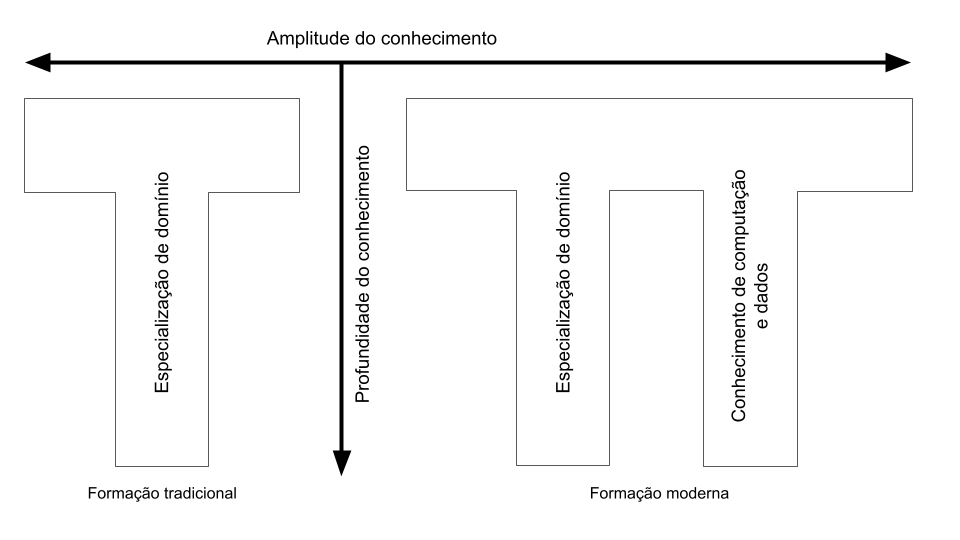
\includegraphics[width=20cm,height=\textheight]{images/pishaped.png}

}

\caption{Perfis profissionais em forma de ``T'' vs forma de ``∏''.
Adaptado de Marwick (2016).}

\end{figure}%

Em 1998, Aldenderfer identificava esta lacuna nos cursos de 1º ciclo na
área da Antropologia nos Estados Unidos da América, dizendo:

\begin{quote}
``Undergraduates, except for the most motivated, are unlikely to ever
see a quantitative class, and therefore, many are poorly prepared for
graduate study. Those who choose to go into cultural resources
management also will be poorly trained, a perennial complaint from the
managers who hire them.'' (Aldenderfer, 1998, p.~108)
\end{quote}

Do lado de cá do Atlântico, e no caso de Portugal em particular, a
situação não é, infelizmente, muito diferente. As páginas que se seguem,
bem como a unidade curricular que representam, são um modesto contributo
para a mudança deste paradigma. Serão, a seu tempo, disponibilizadas
online na íntegra (em conjunto com os ficheiros necessários para a
realização dos exercícios), para que sirvam de suporte a todos os
estudantes que procurem material introdutório sobre análise de dados em
Arqueologia.

\bookmarksetup{startatroot}

\chapter*{\texorpdfstring{\textbf{Introdução}}{Introdução}}\label{introduuxe7uxe3o}
\addcontentsline{toc}{chapter}{\textbf{Introdução}}

\markboth{\textbf{Introdução}}{\textbf{Introdução}}

\section*{\texorpdfstring{\textbf{O registo em Arqueologia: do físico ao
digital}}{O registo em Arqueologia: do físico ao digital}}\label{o-registo-em-arqueologia-do-fuxedsico-ao-digital}
\addcontentsline{toc}{section}{\textbf{O registo em Arqueologia: do
físico ao digital}}

\markright{\textbf{O registo em Arqueologia: do físico ao digital}}

\section*{\texorpdfstring{\textbf{A análise quantitativa em
Arqueologia}}{A análise quantitativa em Arqueologia}}\label{a-anuxe1lise-quantitativa-em-arqueologia}
\addcontentsline{toc}{section}{\textbf{A análise quantitativa em
Arqueologia}}

\markright{\textbf{A análise quantitativa em Arqueologia}}

\part{Dados e Bases de Dados}

\chapter{Tipos de bases de dados}\label{tipos-de-bases-de-dados}

\section{Folhas de cálculo}\label{folhas-de-cuxe1lculo}

\section{Bases de dados relacionais}\label{bases-de-dados-relacionais}

\section{Bases de dados espaciais}\label{bases-de-dados-espaciais}

\chapter{Tipos de dados}\label{tipos-de-dados}

\part{Recolha de dados}

\chapter{Introdução}\label{introduuxe7uxe3o-1}

\chapter{Programa E5}\label{programa-e5}

\part{Transformação de dados}

\chapter{Formatar, ordenar e filtrar}\label{formatar-ordenar-e-filtrar}

\chapter{\texorpdfstring{\textbf{Usar operadores e funções para
transformação de
dados}}{Usar operadores e funções para transformação de dados}}\label{usar-operadores-e-funuxe7uxf5es-para-transformauxe7uxe3o-de-dados}

\section{\texorpdfstring{\textbf{Dados em formato
numérico}}{Dados em formato numérico}}\label{dados-em-formato-numuxe9rico}

\subsection{\texorpdfstring{\textbf{Dados em formato de
texto}}{Dados em formato de texto}}\label{dados-em-formato-de-texto}

\subsection{\texorpdfstring{\textbf{Funções de lógica e de
pesquisa}}{Funções de lógica e de pesquisa}}\label{funuxe7uxf5es-de-luxf3gica-e-de-pesquisa}

\part{Estatística descritiva univariada}

\chapter{\texorpdfstring{\textbf{Tipos de variáveis
estatísticas}}{Tipos de variáveis estatísticas}}\label{tipos-de-variuxe1veis-estatuxedsticas}

\chapter{Variáveis qualitativas}\label{variuxe1veis-qualitativas}

\section{Tabelas de frequência}\label{tabelas-de-frequuxeancia}

\section{Gráficos ou diagramas
circulares}\label{gruxe1ficos-ou-diagramas-circulares}

\section{Gráficos ou diagramas de
barras}\label{gruxe1ficos-ou-diagramas-de-barras}

\chapter{Variáveis quantitativas}\label{variuxe1veis-quantitativas}

\section{\texorpdfstring{\textbf{Medidas de tendência
central}}{Medidas de tendência central}}\label{medidas-de-tenduxeancia-central}

\section{\texorpdfstring{\textbf{Medidas de
dispersão}}{Medidas de dispersão}}\label{medidas-de-dispersuxe3o}

\section{\texorpdfstring{\textbf{Forma da
distribuição}}{Forma da distribuição}}\label{forma-da-distribuiuxe7uxe3o}

\section{\texorpdfstring{\emph{Outliers}}{Outliers}}\label{outliers}

\part{Estatística descritiva bivariada}

\chapter{Duas variáveis
categóricas}\label{duas-variuxe1veis-categuxf3ricas}

\chapter{Uma variável categórica e uma variável
numérica}\label{uma-variuxe1vel-categuxf3rica-e-uma-variuxe1vel-numuxe9rica}

\chapter{Duas variáveis numéricas}\label{duas-variuxe1veis-numuxe9ricas}

\section{Correlação}\label{correlauxe7uxe3o}

\section{Regressão}\label{regressuxe3o}

\bookmarksetup{startatroot}

\chapter*{Bibliografia}\label{bibliografia}
\addcontentsline{toc}{chapter}{Bibliografia}

\markboth{Bibliografia}{Bibliografia}

\phantomsection\label{refs}
\begin{CSLReferences}{0}{1}
\end{CSLReferences}

\bookmarksetup{startatroot}

\chapter*{Anexos}\label{anexos}
\addcontentsline{toc}{chapter}{Anexos}

\markboth{Anexos}{Anexos}




\end{document}
